%-------------------------------------------------------------------------------
% File: simulation.tex
%       Epidemic Broadcast project documentation.
%
% Author: Marco Pinna, Rambod Rahmani, Yuri Mazzuoli
%         Created on 05/12/2020
%-------------------------------------------------------------------------------
\chapter{Simulation}\label{ch:simulation}
As previously described, the scenario considered was the following:
\begin{itemize}
    \item a $100$m x $100$m floorplan, with the transmission
    radius ranging from $1$ m to $19$ m, with a step of $1$ m, and a Bernoullian RV
    with success probability $p$ ranging from $0.1$ to $0.9$ with steps of $0.1$;
\end{itemize}
\section*{Methodological Note}\label{Methodological}
In order to analyse all the possible combinations for $p$ and $R$, it is necessary to explore the space
generated by the cartesian product of the possible values for each parameter. Every combination 
identifies a scenario, performance indexes need to be computed; in the model
every index is a random variable for which the mean value is sought, with appropriate confidence interval
and confidence level (at least 95\%). 
There were not enough details or prior knowledge on the topic to identify the probability distribution of those variables or even to know if they were symmetric.\\
Nevertheless, some \textit{a priori} considerations could be made about their boundedness and therefore variance: all the indexes are clearly bounded from below, being non-negative. In addition:
\begin{itemize}
    \item \textbf{broadcast time} is bounded from below as the broadcast cannot take less than one slot. Moreover, the worst case scenario is given by a single queue configuration with 100 hosts (see \ref{ssec:singlequeue}); the probability distribution for the broadcast time in this type of scenario is the same geometric distribution as the one for a single transmission, scaled up by a factor equal to the number of hops required. This distribution bounds the broadcast time from above and guarantees a finite variance for it.
    \item the \textbf{percentage of covered users} is bounded from above by 1 (100\%).
    \item the \textbf{number of collisions}, in the case of a floorplan with 100 hosts, is bounded from above by the value 2305. The formula for the upper bound can be found in Appendix C, together with its derivation.
\end{itemize} 
This knowledge allowed for the computation of confidence intervals by means of algorithms that do not require to know the distribution of the
samples but only the finiteness of the variance.

For each of the scenarios, the floorplan coverage, the
broadcast duration and the number of collisions are measured and plotted in graphs in order to 
better understand and interpret the behaviour of the system.\\
In order to achieve statistically significant results with a minimum accuracy of
$95$\%, each scenario configuration -- with the same parameters -- was run 200 times; then, mean and median values of the performance
indexes were computed, along with their confidence intervals.

\section{Coverage}\label{ssec:coverage}
Figure \ref{fig:coveragePR} shows the floorplan coverage achieved as a
function of the success probability $p$, for different values of
the transmission radius $R$. \\
As can be observed, the coverage is maximum
for lower values of $p$; this is due to the fact that a low transmission
probability minimizes the number of collisions, increasing the number of correct
transmissions. For values of $R < 8$ we observe an almost linear behaviour:
collisions are almost absent with such a small transmission radius, since the order of the connected component of the graph is quite low; therefore,
variations of the value of $p$ do not play a fundamental role as far as total coverage is
concerned. For $R \geq 8$ the graph starts getting more and more connected and the achievable coverage
decreases with the increase of $p$, but quite slowly and also it does not
degenerate to $0$; instead it reaches a value between $10$\% and $40$\%.
\begin{figure}[H]
    \begin{center}
        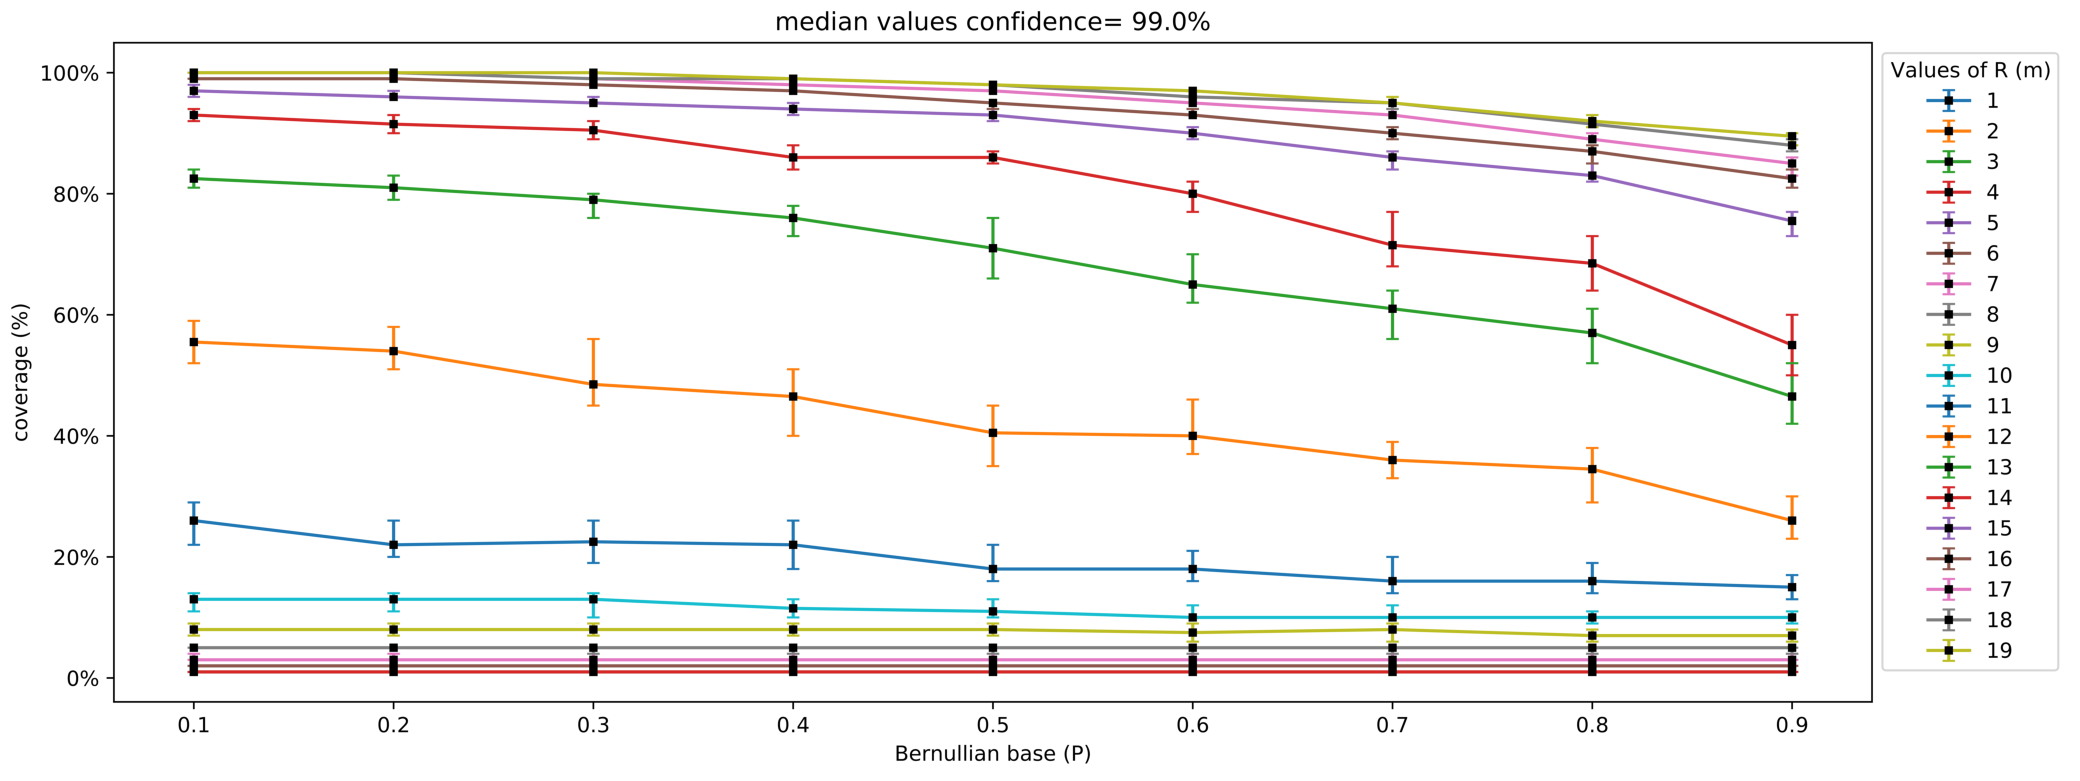
\includegraphics[scale=.42]{img/Big_CovP_median.pdf}
    \end{center}
    \vspace*{-0.5cm}
    \caption{Floorplan coverage as a function of $p$ for different values of $R$}
    \label{fig:coveragePR}
\end{figure}
\noindent
For values of $R$ between $11$ and $15$, the number of collisions has a strong
effect on the coverage percentage; this effect tends to decrease for larger
values of $R$; we know as a matter of fact that for $R \to L\sqrt{2}$ the
coverage tends to $100$\%, independently of any other parameter.\\
\\
Figure \ref{fig:coverageRP} shows the floorplan coverage achieved as a
function of the transmission radius $R$, for different values of the success probability $p$. As expected, accordingly with the previous plot, the
final coverage of the flooplan is deeply influenced by the transmission range $R$.
\begin{figure}[H]
    \begin{center}
        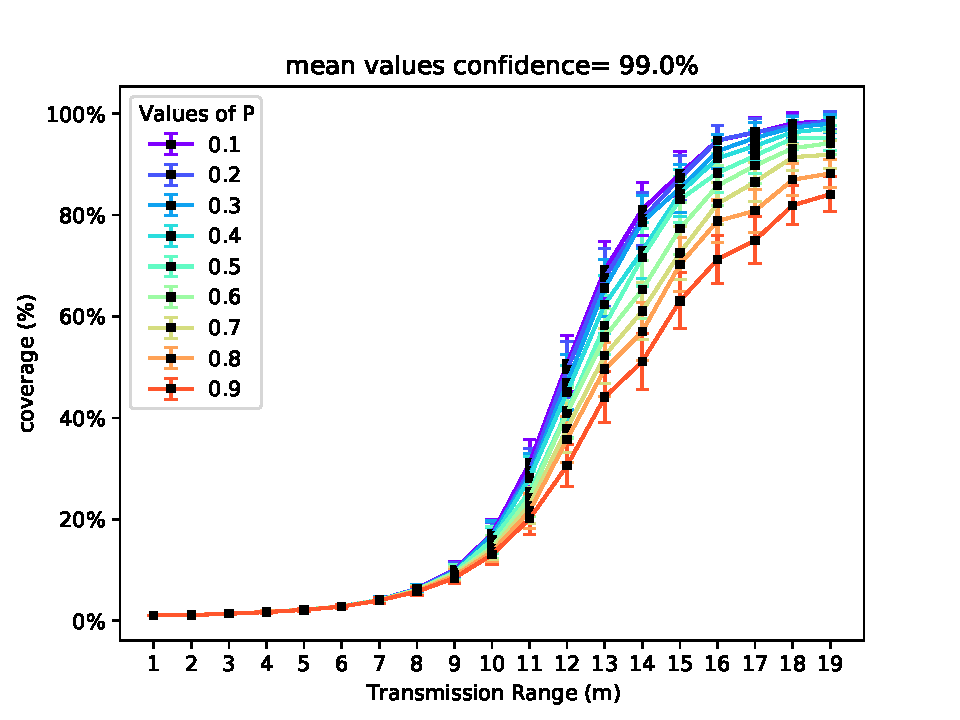
\includegraphics[scale=.75]{img/Big_CovRange_mean.pdf}
    \end{center}
    \vspace*{-0.5cm}
    \caption{Floorplan coverage as a function of $R$ for different values of $p$}
    \label{fig:coverageRP}
\end{figure}
\noindent

In this second plot we can observe that the coverage increases rapidly
with the transmission range, up to about $R=13$ m. When the transmission range becomes large
($> 16$m) there are diminishing returns, as can be seen by the decreasing steepness of the curves, and the coverage tends to a value of 80-100\%, depending on the value of $p$. The coverage function would appear to be a sigmoid, at least for low values of $R$.\\
A more in-depth analysis is carried out in \ref{ssec:coverageReachSafenodes}.
%increasing and can be manipulated to remain between $0$ and $1$ (like the
%parameter we want to fit). A good fit for this curve is given by:
%\begin{equation*}
%    C = \frac{1+\tanh(aR+b)}{2}
%\end{equation*}
%where $C$ is the floorplan coverage, $R$ the transmission radius, and $a$ and
%$b$ depend on $p$ as shown in the following table:
%\begin{center}
%\begin{tabular}{ | m{1cm} | m{4cm}| m{4cm} | }
%\hline
%$p$&$a$&$b$\\
%\hline
%$0.1$&$0.3628314535334378$&$4.356732935967713$\\
%\hline
%$0.2$&$0.3572920723369711$&$4.3206795324164835$\\
%\hline
%$0.3$&$0.34371134773480694$&$4.193385575628803$\\
%\hline
%$0.4$&$0.3217942874156316$&$3.9814759531755515$\\
%\hline
%$0.5$&$0.3091448275788839$&$3.88645016495332$\\
%\hline
%$0.6$&$0.2809863550485405$&$3.6000814495973996$\\
%\hline
%$0.7$&$0.25932462296148107$&$3.3996924196436975$\\
%\hline
%$0.8$&$0.23603288616377227$&$3.1648817545125527$\\
%\hline
%$0.9$&$0.20917405109220505$&$2.929033169711656$\\
%\hline
%\end{tabular}
%\end{center}
\newpage
\section{Collisions}
Figure \ref{fig:collisionsPR} shows the median number of collisions as function of $p$, for different values of $R$.\\
The values seem to have a linear behaviour for low values of $p$ and then start stabilizing as $p$ approaches one.
\begin{figure}[H]
    \begin{center}
        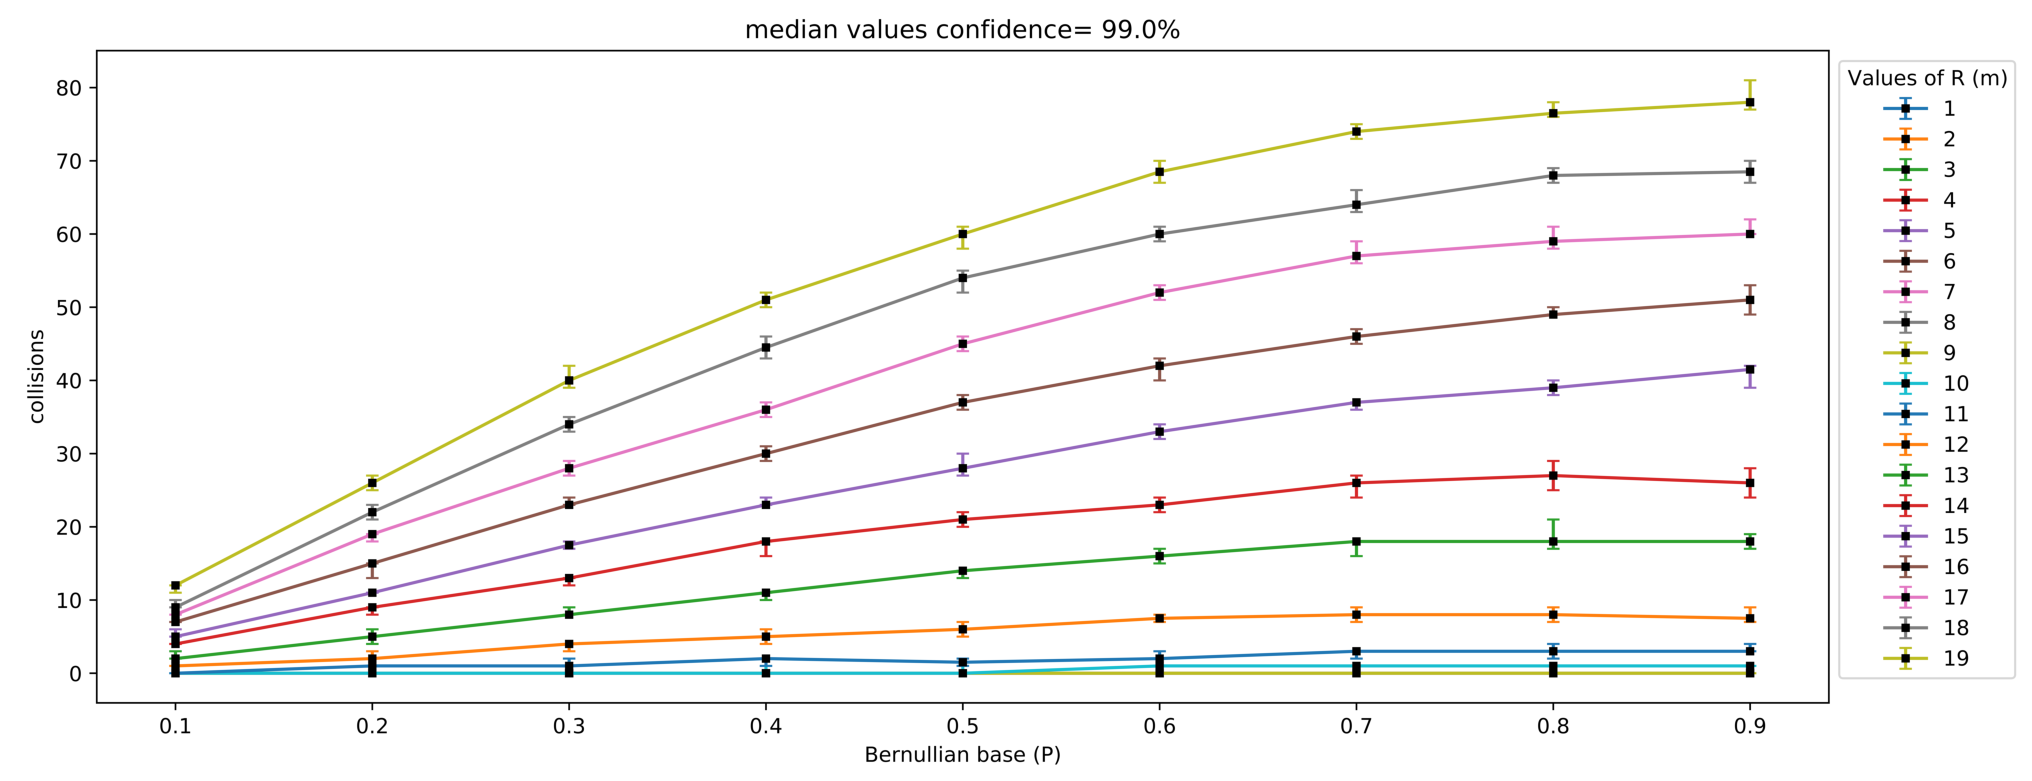
\includegraphics[scale=.45]{img/Big_CollP_median.pdf}
    \end{center}
    \vspace*{-0.5cm}
    \caption{Median value of the number of collisions as function of $R$ for different values of p}
    \label{fig:collisionsPR}
\end{figure}

The dual plot shown in fig. \ref{fig:collisionsRP} provides further insight: low values for $R$ cause no collisions at all, as can also be seen in \ref{fig:collisionsPR} where the lines for $R \leq 8$ all lie on the horizontal axis, regardless of the value of $p$.\\
For bigger values of the radius, the number of collisions grows in a seemingly linear fashion dependent on the value of $R$, with a slope increasing on the increase of $p$.\\
The lines tend to coincide for higher values of $p$, as it also shows the flatness of the curves in the rightmost part of \ref{fig:collisionsPR}.\\
It would incorrect to assert a general positive correlation between the radius and the total number of collisions: as a matter of fact, the number of collisions has to tend to 0 for $R \to \sqrt{2}L$. This is because the more hosts receive the message from host 0, the more of them will be transmitting during the second slot and the less of them will be listening and able to detect a collision.
\begin{figure}[H]
    \begin{center}
        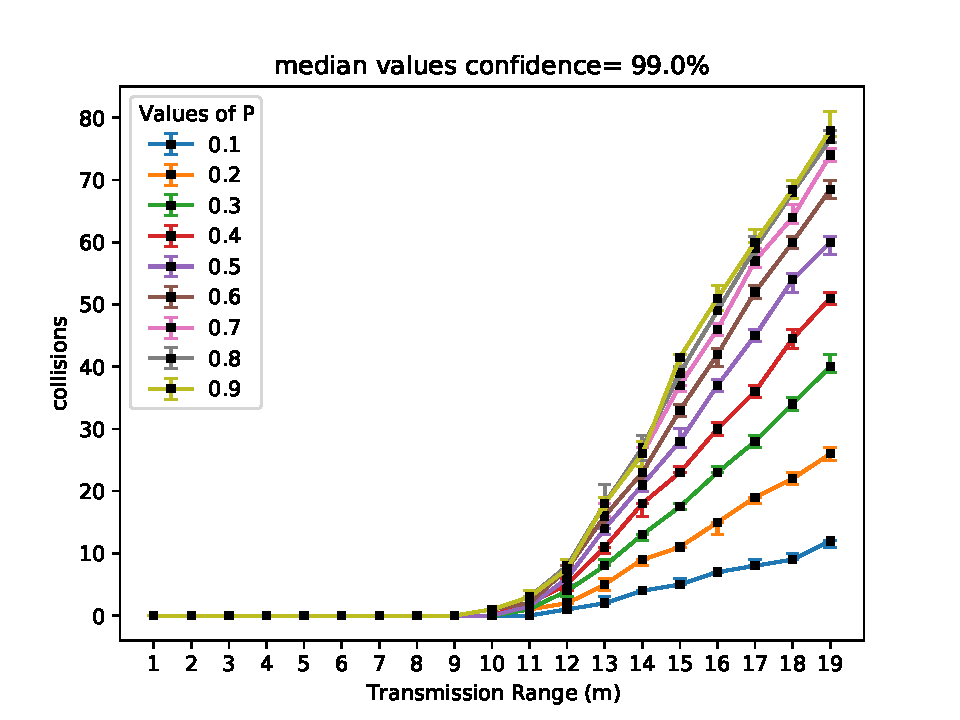
\includegraphics[scale=.6]{img/Big_CollRange_median.pdf}
    \end{center}
    \vspace*{-0.5cm}
    \caption{Median value of the number of collisions as function of $R$ for different values of $p$}
    \label{fig:collisionsRP}
\end{figure}
\section{Duration}\label{sec:duration}
The following figure shows the plot of the duration of the simulation (in
slots) as a function of $p$, for different values of $R$.
\begin{figure}[H]
    \begin{center}
        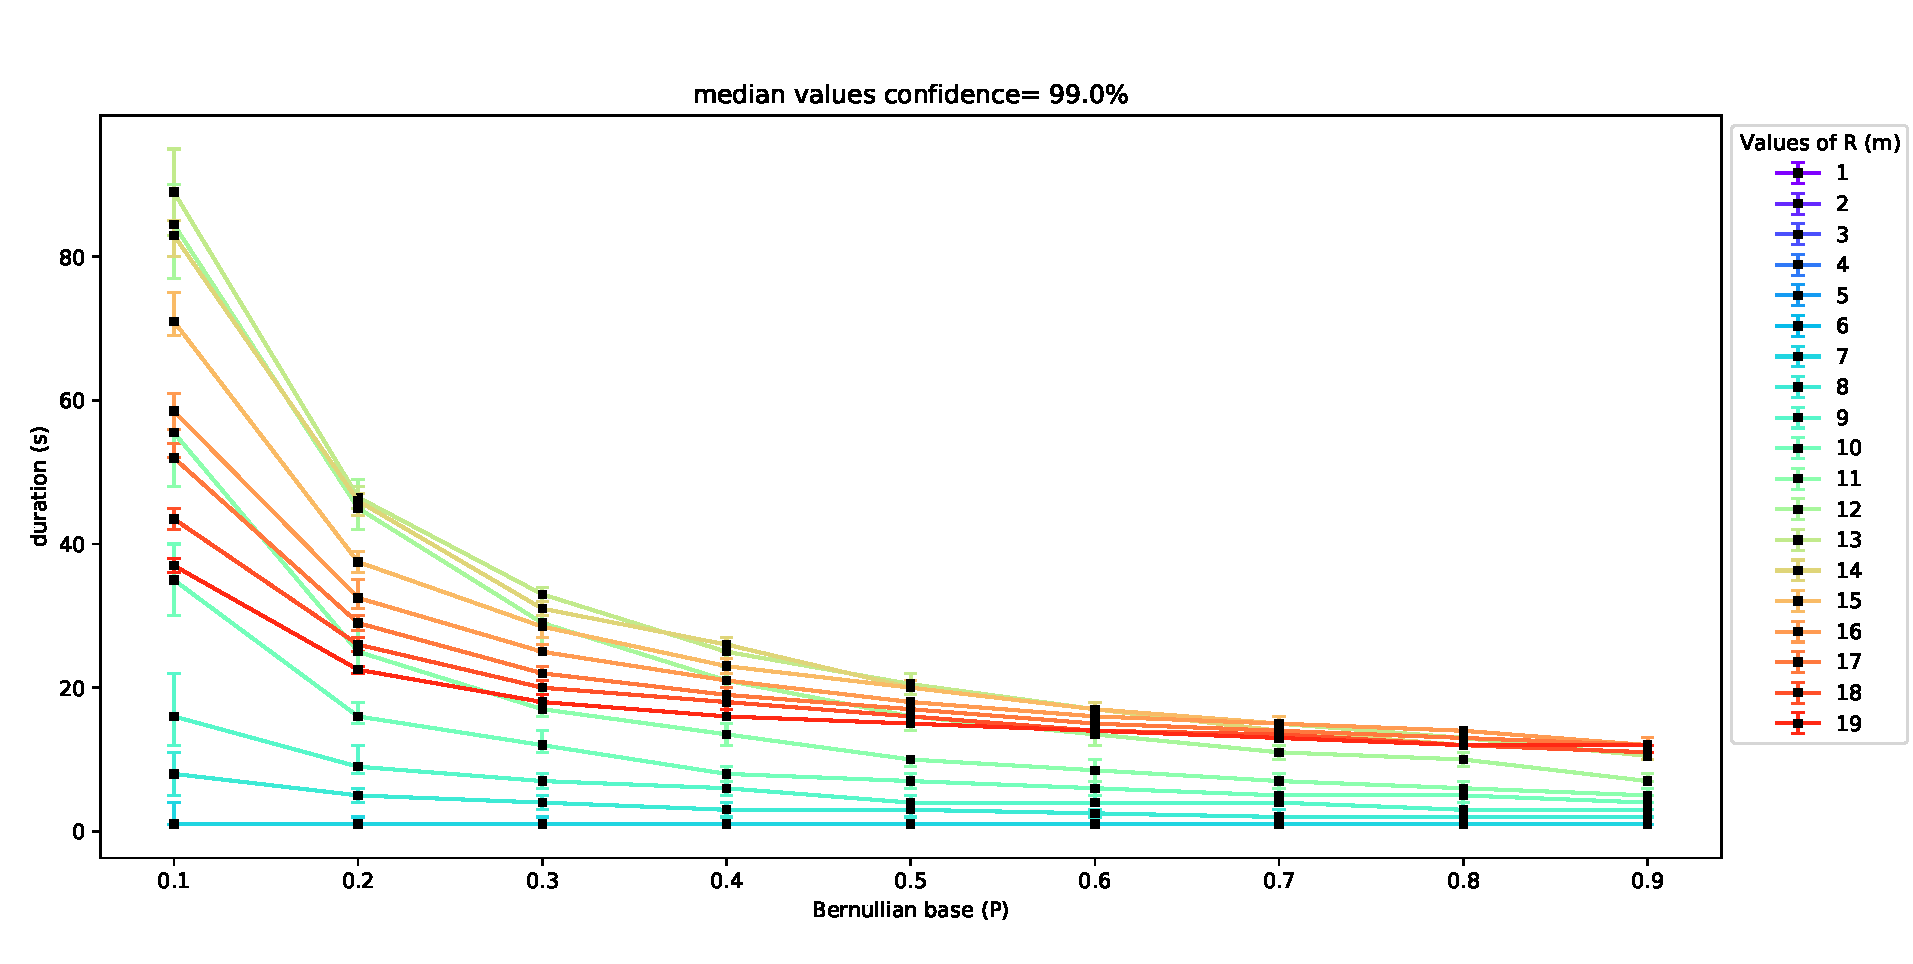
\includegraphics[scale=.45]{img/Big_DurP_median.pdf}
    \end{center}
    \vspace*{-0.5cm}
    \caption{Simulation duration as a function of $p$ for different values of $R$}
    \label{fig:durationPR}
\end{figure}
\noindent
The duration of the broadcast increases for lower values of $p$; this behaviour can be
explained as a consequence of two main factors:
\begin{itemize}
    \item the probability of retransmission is low, hence nodes will spend more
    time slots waiting, without actually transmitting;
    \item with a smaller number of collisions, fewer paths are ``cut off" while the message is travelling along them; this causes the message to stay around for a longer time.
\end{itemize}


\begin{figure}[H]
    \begin{center}
        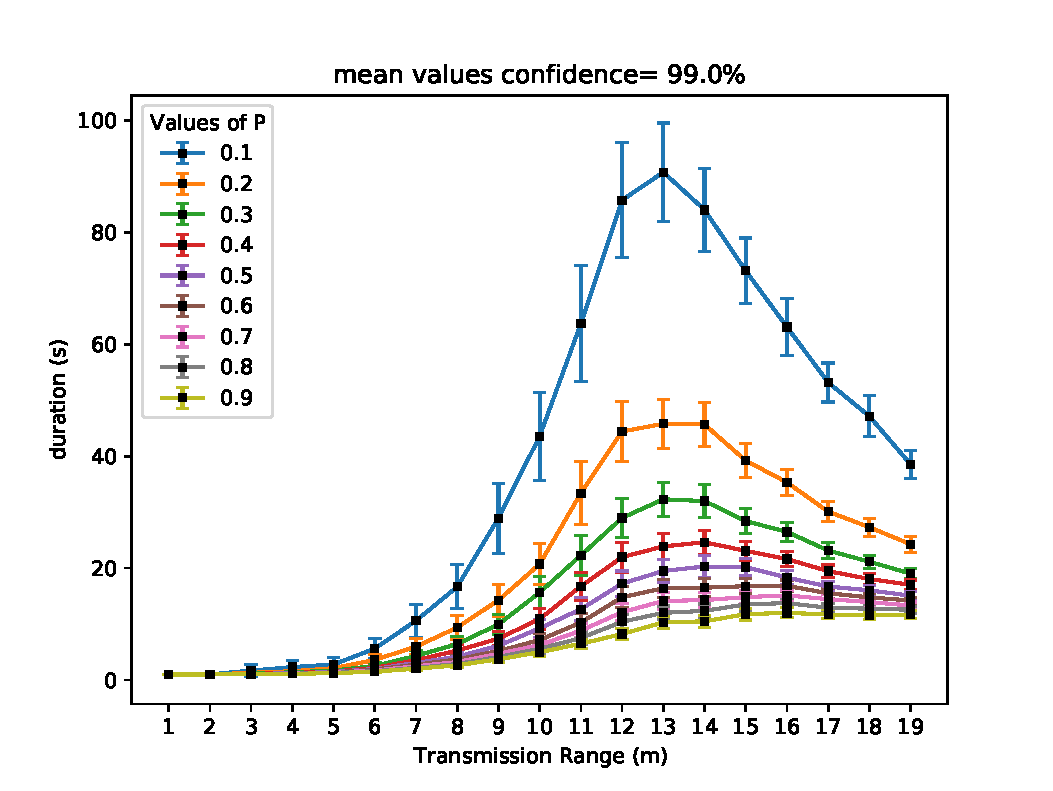
\includegraphics[scale=.6]{img/Big_DurRange_mean.pdf}
    \end{center}
    \vspace*{-0.5cm}
    \caption{Simulation duration as a function of $R$ for different values of $p$}
    \label{fig:durationRP}
\end{figure}
\noindent

The plot in fig. \ref{fig:durationRP} is the dual of the one shown in \ref{fig:durationPR} and shows the duration of the simulation (in slots) as a
function of $R$, for different values of $p$.\\
The duration of the simulation tends to increase with the transmission range,
reaching a peak around $13$ m; the maximum value depends on the probability of
retransmission ($p$) and the distance between the peaks would suggest this dependency to be an inverse proportionality; this would also be consistent with the trend exhibited by the curves in fig. \ref{fig:durationPR}, where the topmost ones resemble hyperbolas.\\
The bottom ones are much flatter, since very low values of $R$ often do not even allow the starting node to be connected to any others.
This supposedly inverse proportionality with respect to $p$ is an interesting result and can be explained by observing that the same inverse proportionality is found in formula \ref{eq:singleQueueMeanT}.\\
Further observation about this and relationship with some graph properties are discussed in \ref{ssec:durationVsEccentricity}.\\
Not all the curves in \ref{fig:durationPR} exhibit a hyperbolic trend: very low values of $R$ cause them to have a degenerate trend, while for high values of $R$ the deviation from the hyperbola is probably due to the increasing influence of the collision.

We tried to interpolate the curves shown in Figure \ref{fig:durationPR}
with an hyperbolic function, because it fits well the parameters we want to
model; first of all, the hyperbole tends to infinity as $p$ tends to $0$, and
this is coherent with the reality, because if the probability of retransmission
becomes low, then the duration keeps increasing. If instead $p$ gets close to
$1$, the duration time tends to its minimum. We fit those shapes using:
\begin{equation*}  
    D = \frac{a}{P}+b 
\end{equation*}
where $D$ is the duration of the simulation, $p$ the probability of
retransmission, and $a$ and $b$ depend on $R$ as specified in the following
table:
%TODO too many digits. Better to reformat as the wall of text is not exactly pretty
%\begin{center}
%\begin{tabular}{ | m{1cm} | m{5cm}| m{5cm} | }
%\hline
%$R$&$a$&$b$\\
%\hline
%$1$&$2.4046845625846913$ e-09&$0.999999999244136$\\
%\hline
%$2$&$2.4046845625846913$ e-09&$0.999999999244136$\\
%\hline
%$3$&$0.7313966348173997$&$0.9495446821974095$\\
%\hline
%$4$&$1.3471717522270503$&$0.9454326532617134$\\
%\hline
%$5$&$1.7744177255115228$&$1.08724762049118$\\
%\hline
%$6$&$4.652279267805434$&$1.0487610714204172$\\
%\hline
%$7$&$9.586489452244717$&$1.088347295851843$\\
%\hline
%$8$&$15.841670397411658$&$1.0643797063994824$\\
%\hline
%$9$&$28.264640360031194$&$0.49558107430696624$\\
%\hline
%$10$&$43.141734847778814$&$0.22815570364285975$\\
%\hline
%$11$&$64.55944043148898$&$-0.07517936077209139$\\
%\hline
%$12$&$86.56257725232254$&$-0.09919809415424388$\\
%\hline
%$13$&$89.72686483087844$&$1.2578386401845827$\\
%\hline
%$14$&$82.15919574473708$&$3.0965825999956778$\\
%\hline
%$15$&$67.95268283187643$&$5.415446394742158$\\
%\hline
%$16$&$56.442159145137495$&$6.991880399220213$\\
%\hline
%$17$&$45.71412729773696$&$7.548465010848107$\\
%\hline
%$18$&$39.164500694866284$&$7.991652317096266$\\
%\hline
%$19$&$29.71836400235831$&$9.075854630828385$\\
%\hline
%\end{tabular}
%\end{center}
as a matter of fact, if the transmission range is
too short nodes can not communicate: they are not in reach by each others.\\
\\

\section{Comparison between KPIs and graph properties}

Some of the results shown in the previous section can be better understood when compared with some properties of the graphs associated with the configurations of the hosts.\\
In particular, three properties of the graphs have been studied:

\begin{itemize}
	\item the \texttt{reach}, defined as the number of nodes that can be reached from host (vertex) 0. More formally, let $H$ be the connected component containing host 0 of the initial graph $G$, i.e. the induced subgraph in which any vertex is connected to vertex 0. The \texttt{reach} is the \textit{order} of $H$.
	\item the \texttt{eccentricity}, already defined in \ref{sec:graphModelForWirelessSystems}
	\item the number of \texttt{safe nodes}, which has been defined for simulations with $p=1$ as the number of nodes that correctly receive the message. Systems with $p=1$ are completely deterministic and therefore the number of \textit{safe nodes} only depends on the topology of the network.
\end{itemize}

\subsection{Coverage, reach and safe nodes}\label{ssec:coverageReachSafenodes}

In \ref{ssec:coverage} results about the coverage were shown and it was hypothesized that this index, as function of $R$, might have a sigmoidal trend.\\
Let us consider the limit case where $p \to 0$.\\
As $p$ approaches 0, during each slot it becomes less and less likely for an active node to transmit the message. On the other hand, smaller values of $p$ lower the probability of collisions even more.\\
For values of $p$ really close to 0, it is easy to imagine that there will be basically no collisions; at the same time, every node belonging to the connected component of node 0 will sooner or later receive the message with a probability of 1.\\
\begin{figure}[H]
	\begin{minipage}{.5\textwidth}
        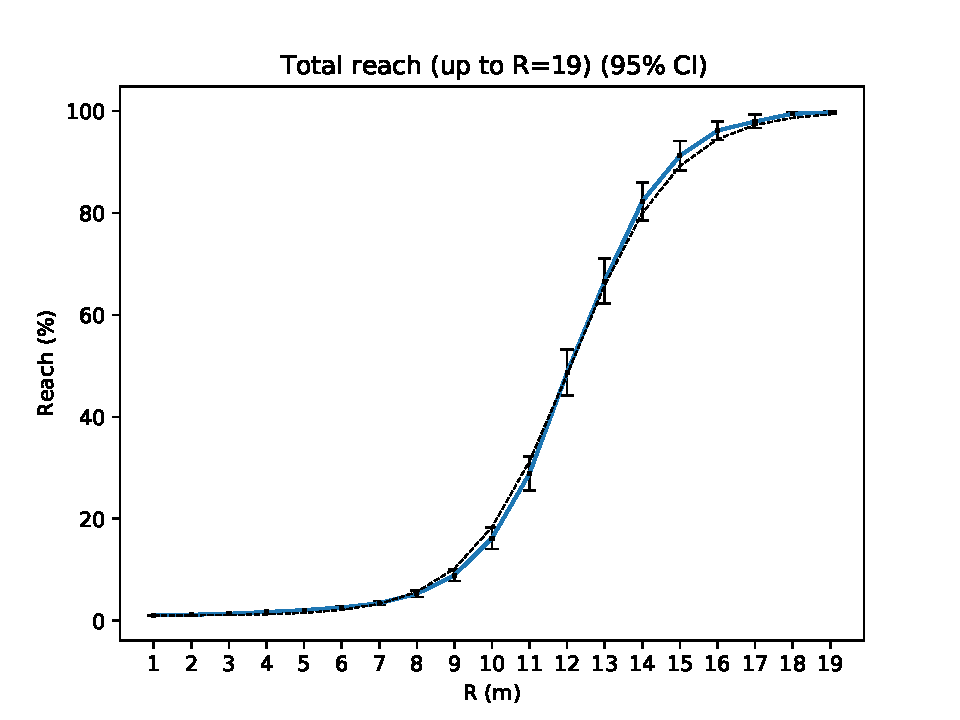
\includegraphics[scale=.5]{img/graphAnalysisTotal_reachR19.pdf}
        \begin{center}
            a)
        \end{center}
	\end{minipage}
	\begin{minipage}{.5\textwidth} 
		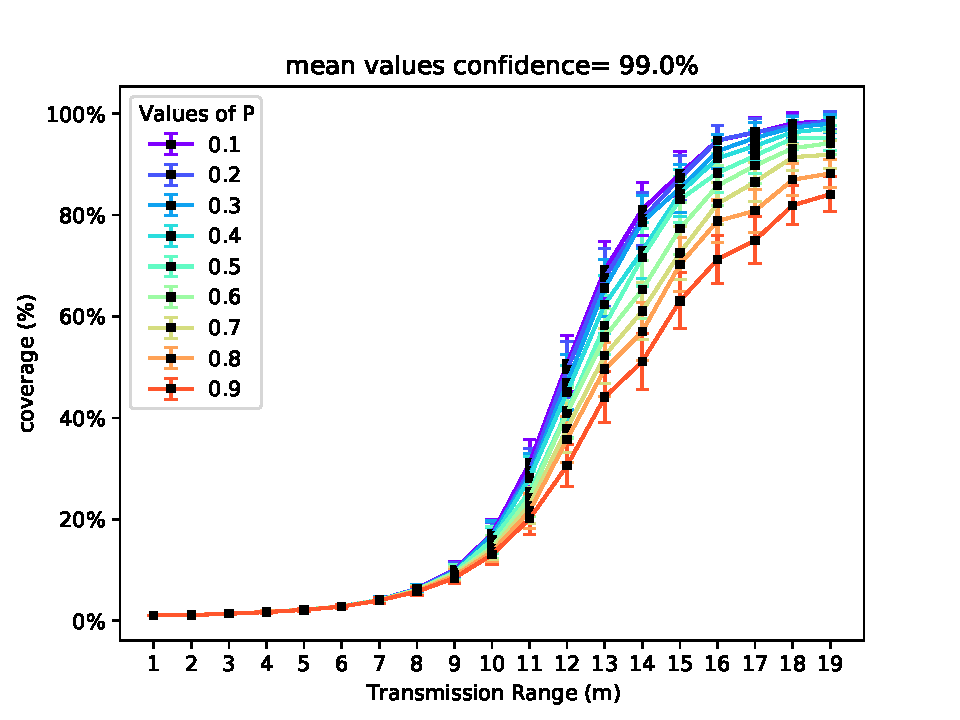
\includegraphics[scale=.5]{img/Big_CovRange_mean.pdf}
		\begin{center}
            b)
        \end{center}
	\end{minipage}
	\caption{}
    \label{fig:reachR30}
\end{figure}
\hfill \break
\hfill \break
Figure \ref{fig:reachR30} a) shows the average reach from node 0, as function of $R$, in a graph with 100 nodes and figure \ref{fig:reachR30} b) the experimental data for the coverage, for convenience of comparison. The plot in \ref{fig:reachR30} a)  plateaus at a value of 100 for values of $R \geq24$ metres. \\
Various sigmoid functions have been tested to fit the experimental values for the \textit{reach}, and the most appropriate one was found to be
\hfill \break
\begin{equation}\label{eq:reachSigmoidParametric}
	S(R) = \frac{1}{N} + \frac{N-1}{N}\cdot\frac{1+tanh(b(R-a))}{2}
\end{equation}
\hfill \break
where $N$ is the number of nodes in the graph, $a$ controls to the abscissa of the inflection point and $b$ controls how steep the increase is.\\
The correct value for $a$ can be found examining the data in fig. \ref{fig:reachR30} and observing that they show an inflection point for $R=12$ m. With regard to parameter $b$, trial and error showed that its value lies between $0.36$ and $0.37$. In fact, a value equal to $e^{-1} \approx 0.36788$ fits the data very well.\\
% and it makes sense in the presence of a hyperbolic tangent function ?
A closed form for the \textit{reach}, and therefore for total coverage when $p \to 0$, in a square floorplan with $L=100$ would then be
\hfill \break
\begin{equation}\label{eq:reachSigmoidNoL}
	C_{0}(R) = \frac{1}{100} + \frac{99}{100}\cdot\frac{1+tanh(e^{-1}(R - 12))}{2}
\end{equation}
\hfill \break
This formula, however, models the coverage for a fixed values of \texttt{L} and $N$, as mentioned above.\\
A more complete closed form, that also takes in account the length of the side of the floorplan and the number of hosts, could be the following:
\hfill \break
\begin{equation}\label{eq:reachSigmoidL}
	C_{0}(R, L, N) = \frac{1}{N} + \frac{N-1}{N}\cdot\frac{1+tanh(e^{-1}(10\sqrt{N}\frac{R}{L} - 12))}{2}
\end{equation}
\hfill \break
The presence of the quantity $\frac{R}{L}$ follows from the observation that the overall connectivity of a graph should only depend on the ratio between the transmission radius and the coordinates of the hosts (see section \ref{sec:graphModelForWirelessSystems}).\\
The rationale behind the $\sqrt{N}$ term is that the average number of nodes per unit area goes with the \textbf{square} of $N$, and supposedly also does the average number of nodes per transmission circle.\\
Another way to visualize this is to imagine the entire graph in a $L$x$L$ floorplan, divide the floorplan in four $\frac{L}{2}$x$\frac{L}{2}$ squares and take the graph that lies in one of these squares: on average it will have a fourth of the initial number of nodes but its level of connectivity should presumably be the same as the original graph.\\
The value for $a$, as mentioned above, was found by observing experimental data and it is, almost certainly, not an exact value.\\
Lastly, coverage is also likely to depend on the shape of the floorplan itself, which is not taken in account in the formula. Further research is needed\\
\hfill \break
Let us now consider the limit case where $p \to 1$.\\
The closer $p$ gets to $1$, the more the system approaches a deterministic behaviour where each active host broadcasts the message as soon as it receives it.\\
When $p=1$ the number of node that correctly receive the message during the broadcast can be computed by knowing only the topology of the network.\\
\begin{figure}[H]
    \begin{center}
        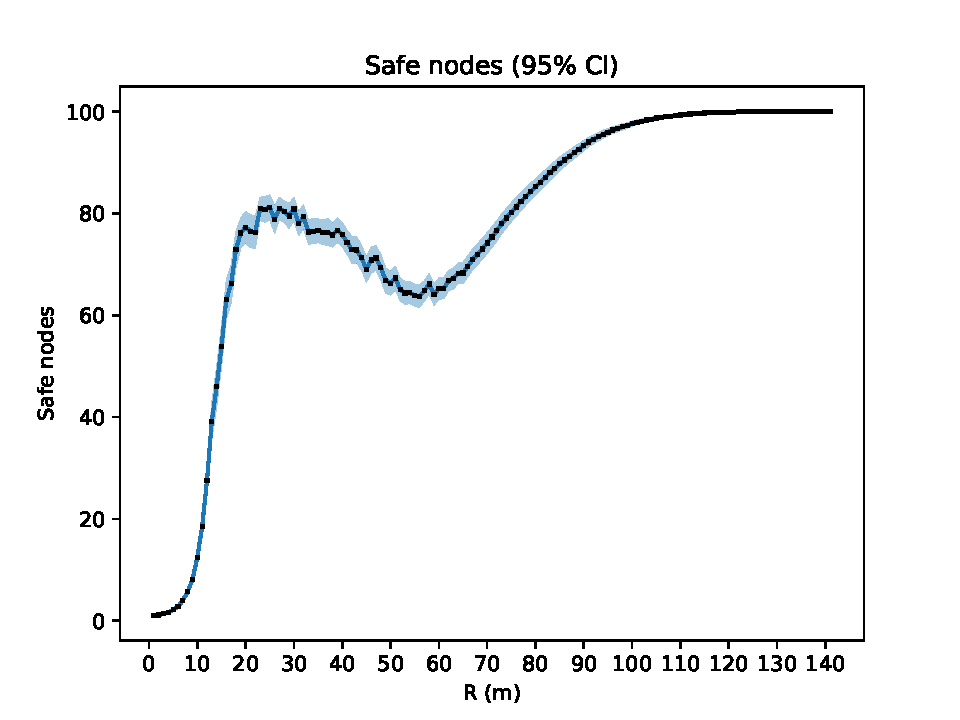
\includegraphics[scale=.6]{img/graphAnalysisSafe_nodes.pdf}
    \end{center}
    \vspace*{-0.5cm}
    \caption{Average number of safe nodes of a graph as function of R}
    \label{fig:safeNodes}
\end{figure}
\hfill \break
Figure \ref{fig:safeNodes} shows the average number of safe nodes during a broadcast starting from node 0, as function of $R$, in a graph with 100 nodes.\\
It is clear that this function does not have a sigmoidal trend, except for low values of $R$, up to about 25 metres, where the number of safe nodes reaches about 80. This is consistent with the trend of the curve for $p=0.9$ in Figure \ref{fig:coverageRP} shown in the previous section.\\
For $R > 25$, increasing the radius yields negative returns: the average number of safe nodes decreases until $R$ reaches about 55 metres. This is likely to be due to the fact that the increase in the number of collision takes over on the increase of reachable nodes. This is consistent with the hypothesis made in Chapter \ref{ch:overview} when analysing the impact of $R$ on the KPIs.\\
For $R > 55$ the number of safe nodes starts increasing again, probably because host 0 starts having more and more neighbours when the broadcast begins (and none of them detects a collision as host 0 is the only one transmitting during the first slot).\\ The quantity asymptotes to the total number of nodes and for $R > \sqrt{2}{\cdot}L$ it is identically equal to it since, wherever the starting node would happen to be placed, it would cover the whole area during its first transmission slot.\\
\hfill \break
These considerations show that the coverage as function of $R$, although it might resemble a sigmoid for different values of $p$ (and could probably be approximated well enough by it for realistic value of the transmission range), is probably more complex than that; for a certain range of values for R, the increase in the number of collision starts having a heavier role in the number of reached hosts.\\
A closed formula for the number of safe nodes when $p=1$ has not been found yet but, assuming it is $C_{1}(R)$, then a reasonable form for the coverage function could be the following:
\begin{equation}\label{eq:coverageClosedForm}
C(R, p) = (1-p)\cdot C_{0}(R) + p\cdot C_{1}(R)
\end{equation}
\newpage
\subsection{Broadcast time and eccentricity}\label{ssec:durationVsEccentricity}
In \ref{sec:graphModelForWirelessSystems} the eccentricity $\epsilon$ of a graph was introduced, defined as the distance from node 0 to the furthest connected node, let it be $u$.\\
If we imagine the message spreading from host 0 outwards along the various paths of the graph, it is easy to guess that, on average, the path that will take the longest to be covered will be the one that leads to node $u$ and this path will have, by definition, a number of edges equal to the eccentricity.\\

\begin{figure}[H]
    \begin{center}
        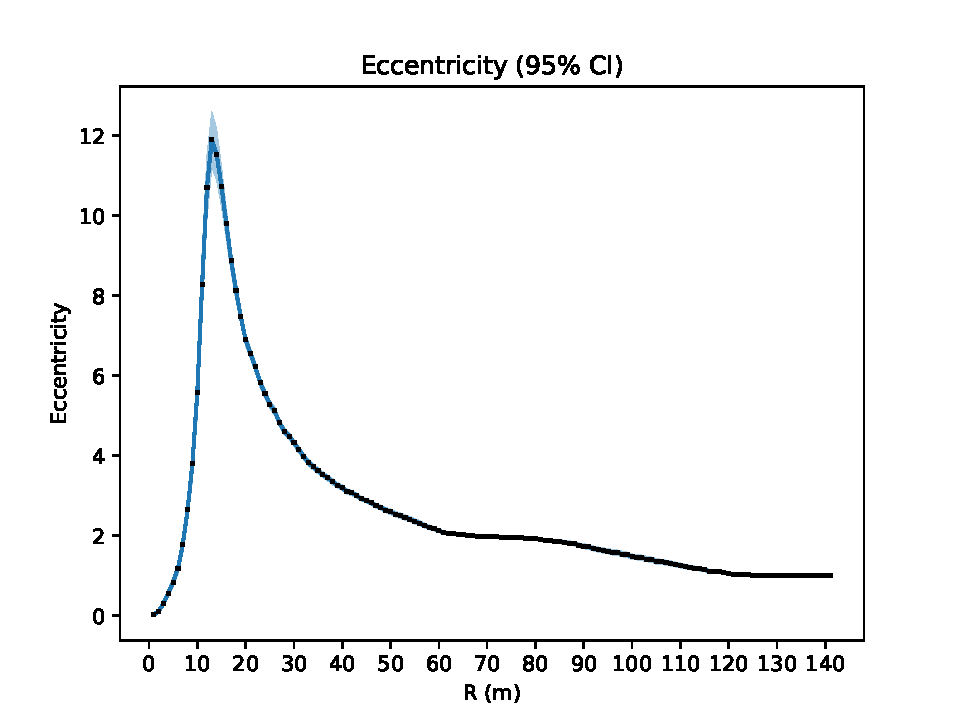
\includegraphics[scale=.6]{img/graphAnalysisEccentricity.pdf}
    \end{center}
    \vspace*{-0.5cm}
    \caption{Average number of safe nodes of a graph as function of R}
    \label{fig:eccentricityFull}
\end{figure}
\hfill \break
Figure \ref{fig:eccentricityFull} shows the average eccentricity of a graph with 100 nodes, as function of R.
The function has a maximum around $R = 13$ m and then starts slowly decaying until it reaches 1 as R gets closer to $\sqrt{2}L$; this makes complete sense since, for high values of R, node 0 is quite likely to be connected to all nodes in the floorplan.\\
The peak at $R=13 m$ has the following physical interpretation: for values of R between 0 m and 13 m, increasing the radius increases the order of the connected component of the graph containing node 0; by further increasing the radius, more edges start to appear in the graph creating shorter paths between nodes that were already connected.\\
Another interesting observation concerns the behaviour of the function around $R = 70$ m: the eccentricity seems to stabilize at a value of 2, with very narrow confidence intervals, for values  of $R$ close to $\frac{1}{2}\sqrt{2}L$.\\
Fig. \ref{fig:eccentricityDuration} shows the previous function up to $R=19$ m one one side, and again the experimental data for the duration, for convenience of comparison.\\
\begin{figure}[H]
	\begin{minipage}{.5\textwidth}
        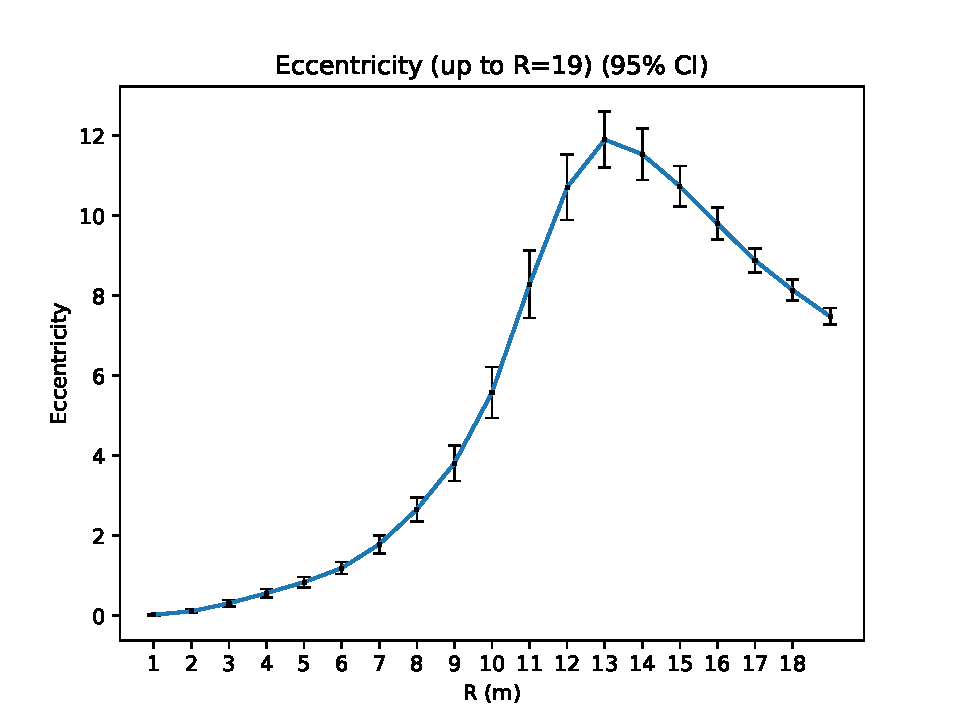
\includegraphics[scale=.5]{img/graphAnalysisEccentricityR19.pdf}
        \begin{center}
            a) Eccentricity as function of R
        \end{center}
	\end{minipage}
	\begin{minipage}{.5\textwidth} 
		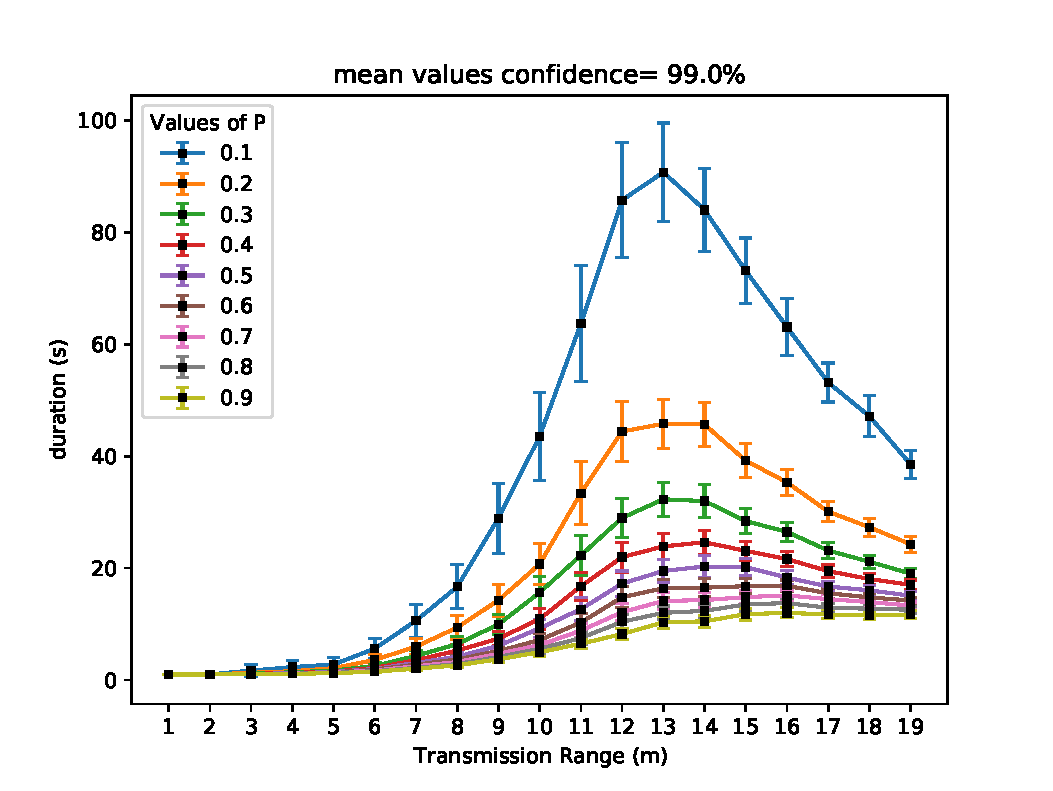
\includegraphics[scale=.5]{img/Big_DurRange_mean.pdf}
		\begin{center}
            b) Broadcast time as function R
        \end{center}
	\end{minipage}
	\caption{}
    \label{fig:eccentricityDuration}
\end{figure}
\hfill \break
The curves on the right clearly resemble the one on the left, minus a scaling factor, especially for lower values of $p$.\\
As the value of $p$ approaches one, the curves tend to flatten and this might be due to the fact that the number of collision increases and more paths are cut off (see \ref{sec:duration}).\\
The spacing between the duration curves might suggest that this scaling factor is the inverse of the corresponding $p$, as mentioned earlier. This would make complete sense because the average time a message takes to travel along a path of $n$ hops is $n \cdot \frac{1}{p}$ (see \ref{ssec:singlequeue}).\\
In fact, while the spacing does indeed suggest an inverse dependency on $p$, the actual values turn out to be about 20\% smaller. The existence of this additional $\sim0.8$ scaling factor could be motivated as follows:\\
the eccentricity of a graph gives information about the longest path from a node to the furthest node $u$, but does not say anything about the number of paths of that length. In the graph there might very well be different paths of length $\epsilon$ that connect node 0 to $u$, either completely disjunct or with some nodes in common and ``forks", ``branch-ins" and ``branch-outs". If these paths happens to be disjunct, node $u$ will receive the message as soon as it arrives from the ``fastest" one. 

\begin{wrapfigure}{r}{0.45\textwidth}

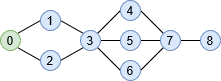
\includegraphics[width=1\linewidth]{img/branchIn.png} 
\caption{Example of graph with multiple shortest path of lenght $\epsilon$}
\label{fig:branchIn}
\end{wrapfigure}

If the paths happen to have nodes in common, as it is the case in fig. \ref{fig:branchIn}, every time there is a ``branch-in" ($[1,2]{\to}3$ or $[4,5,6]{\to}7$ in the figure) there is a possibility that the message will have a speed ``boost" with respect to its average speed along a single queue and also a possibility that its progress will be interrupted by a collision.

\section{Performance optimization}
The ultimate goal of this study is to find the optimal configuration of parameters to ensure the highest coverage in the lowest possible time, since the message should ideally reach all the users as soon as possible.\\
The trivial solution is to make the transmission radius so big that it covers the entire floorplan, thus ensuring total coverage in one single slot.
This is clearly not viable if the floorplan size gets really big.\\
If one wishes to only maximize the coverage, regardless of the amount of time it would take to reach the last user, they should choose the biggest $R$ the devices allow for and a low value of $p$: this configuration corresponds to the top right corner of figure \ref{fig:coverageRP}. The downside of this choice of parameters is that the duration of the broadcast will be very long, as shown in the corresponding curve in fig. \ref{fig:durationRP}.\\
If, instead, one wishes to minimize the duration of the broadcast, possibly at the expense of not having full coverage, they should opt for a higher value of $p$. In this case, the choice of $R$ is not as obvious: provided that $R$ cannot be large enough to cover the whole area, it should be ensured that chosen value does not fall within the range that yields negative returns, as discussed in the second part of \ref{ssec:coverageReachSafenodes} and shown below in fig. \ref{fig:safeNodesShaded}. In practical terms, referring to fig. \ref{fig:safeNodes}, if $R$ can be greater than $\sim76$ metres, it should be as high as possible; if it cannot be greater than $\sim76$ metres, then $R$ should be kept at $\sim25$ metres, since higher values would result in a poorer performance.

\begin{figure}[H]
    \begin{center}
        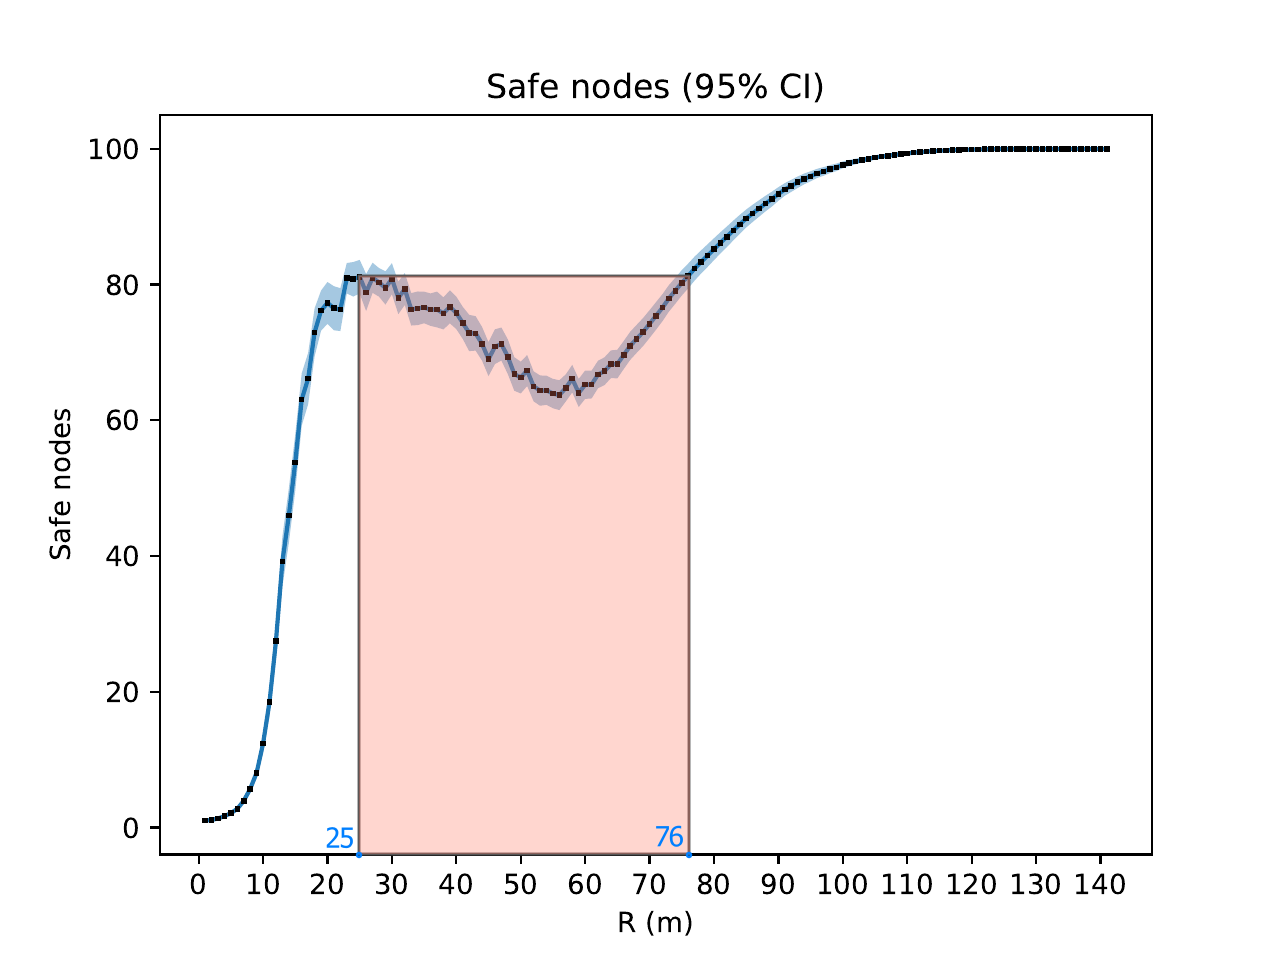
\includegraphics[scale=0.7]{img/graphAnalysisSafe_nodesRed.png}
        \caption{}
        \label{fig:safeNodesShaded}
    \end{center}
    \vspace*{-0.8cm}
\end{figure}